% если хочется, можно поставить 14pt
\documentclass[12pt, dvipsnames]{extarticle}

\usepackage{luatex85}
\pdfminorversion=5

\usepackage{fontspec}
\usepackage{polyglossia}
\usepackage[a4paper, 
lmargin=30mm, rmargin=15mm, tmargin=20mm, bmargin=20mm]{geometry}
\usepackage{multirow}

\usepackage{pgfplots}
\pgfplotsset{compat=1.18}

\setdefaultlanguage{russian}
\setotherlanguage{english}

% Согласно требованиям к ВКР
\defaultfontfeatures{Ligatures=TeX}

\setmainfont{Times New Roman}
\setmonofont{Courier New}
\setsansfont{Arial}

\newfontfamily\cyrillicfont{Times New Roman}
\newfontfamily\cyrillicfontsf{Arial}
\newfontfamily\cyrillicfonttt{Courier New}

\newfontfamily\englishfont{Times New Roman}
\newfontfamily\englishfontsf{Arial}
\newfontfamily\englishfonttt{Courier New}

\linespread{1.5}

\usepackage{titlesec}

\titleformat{\section}{\normalfont\fontsize{14}{14}\bfseries}{\thesection}{1em}{}
\titleformat{\subsection}{\normalfont\fontsize{14}{14}\bfseries}{\thesubsection}{1em}{}
\titleformat{\subsubsection}{\normalfont\fontsize{14}{14}\bfseries}{\thesubsubsection}{1em}{}

\setlength{\parindent}{1.25cm}

\renewcommand\thesection{\arabic{section}}

\usepackage[a-1b,mathxmp]{pdfx}
\hypersetup{hidelinks,colorlinks=true,citecolor=BurntOrange,urlcolor=Blue}

\usepackage[backend=biber,
bibencoding=utf8,
sorting=none,
style=gost-numeric,
language=autobib,
autolang=other,
clearlang=true,
defernumbers=true,
sortcites=true,
doi=true,
isbn=true,
]{biblatex}

\renewcommand{\UrlFont}{\small\rmfamily\tt}
\appto{\bibsetup}{\raggedright}

\bibliography{bibliography/betti}
%\bibliography{bibliography/}


\usepackage{amsfonts}

\usepackage{tikz}
\usepackage{pgfplots}
\usepackage{wrapfig}

\usepackage{caption}
\usepackage{subcaption}

\usepackage{amsfonts, amssymb, amsmath, amsthm}
\usepackage{mathtools}
\usepackage{enumerate}
\usepackage{verbatim}

\usepackage{mathrsfs,amsfonts,mathtools}
\usepackage{amsmath}          
\usepackage{amssymb}

\usepackage{amsthm} 
\usepackage{thmtools}
\usepackage{array}

\usepackage{graphicx} 
\graphicspath{{images/}}

\renewcommand{\emptyset}{\varnothing}
\renewcommand{\epsilon}{\varepsilon}
\renewcommand{\phi}{\varphi}
\renewcommand{\kappa}{\varkappa}

\begin{document}
	\setcounter{page}{2}
	
	\vspace*{\fill}
	\begin{abstract}
		В работе ставится задача извлечения пользовательских атрибутов из диалоговых реплик в структурированном формате, для дальнейшего использования их в персонализованных диалоговых агентах или в рекомендательных системах. Из-за отсутствия данных с качественной разметкой, используется техника разметки c помощью моделей из других задач, добавляющая шум в данные. Предлагаются два способа решения поставленной задачи на основе трансформеров: решение с одной моделью (GenAE) и с двумя моделями (PipelineAE). Обсуждаются недостатки и преимущества обоих подходов. По итогу проведенных экспериментов получены результаты выше чем у существующих подходов решения данной задачи. Предложены методы улучшения качества разработанного framework'a и направления для дальнейших исследований.
	\end{abstract}
	\vspace*{\fill}
	
	\newpage
	\tableofcontents
	
        \newpage
	\chapter{\centering{\normalsize{ОПРЕДЕЛЕНИЯ, ОБОЗНАЧЕНИЯ И СОКРАЩЕНИЯ}}}
\addcontentsline{toc}{section}{ОПРЕДЕЛЕНИЯ, ОБОЗНАЧЕНИЯ И СОКРАЩЕНИЯ}

В настоящем отчете о НИР применяют следующие сокращения и обозначения:

Авторегрессионная генеративная модель --- модель генерирующая следующий элемент входной последовательности, неявно используя условное распределение следующего элемента по предыдущим.

Метод k-ближайших соседей (англ.: k-nearest neighbors algorithm, kNN) --- алгоритм для автоматической классификации объектов или регрессии.

Персона --- описание личности в разговорных диалоговых датасетах. Обычно состоит из 5-6 коротких предложений о пользователе и его предпочтениях.

Трансформер (англ.: Transformer) --- архитектура глубоких нейронных сетей, использующая механизм внимания для повышения скорости обучения.

Триплет --- кортеж из трех элементов: (субъект, отношение, объект). Отношение или предикат определяется из конечного множества.

Batch --- подмножество объектов из всего датасета, которое обычно выбирается случайно. Используется в обучении современных больших нейронных сетей с помощью стохастического градиентного спуска или Adam.

BERT (сокращ.: Bidirectional Encoder Representations from Transformers, рус.: двунаправленные векторные представления трансформера) --- архитектура и метод предобучения трансформера, при котором модель должна предсказать токены последовательности, замененные на специальный MASK-токен, а также, является ли второе предложение из двух поданных на вход продолжением первого в тексте.

Checkpoint --- промежуточные сохраненные веса модели во время обучения для фиксации состояния обучения.

Сollaborative filtering --- подход к построению рекомендательных систем, при котором контент/товары рекомендуются на основании схожести пользователей. 

Сontent-based filtering --- подход к построению рекомендательных систем, при котором пользователи сопоставляются с контентом или товарами, которые им нравятся.

Distant supervision --- прием использующийся в построении графов знаний. Основная идея и предпорложение приема заключается в том, что если какие то две сущности находятся в определенном отношении, то любое предложение содержащее эти сущности выражает это отношение.

Encoder-decoder --- архитектура моделей которые решают задачи sequence-to-sequence. Encoder получает некоторые представление входных данных, а decoder преобразовывает это представление в выходные данные.

Few-shot --- разновидность обучения с учителем, когда обучающих примеров чрезвычайно мало: обычно 5 или 1.

Framework --- комплексное программное обеспечение которое содержит в себе методы преобразования данных и обучение моделей вместе с методами оценки их качества.

Gated Recurrent Unit (сокращ.: GRU, рус.: управляемый рекуррентный блок) --- разновидность архитектуры рекуррентных нейронных сетей, обладающая улучшенными свойствами обработки долговременных последовательностей, но при этом имеющая меньшее число параметров по сравнению с LSTM.

GBDT (Gradient Boosting Decision Tree) --- алгоритм дерева решений, основанный на итеративном накоплении.

Logit --- выходные данные модели до применения активации Sigmoid или Softmax.

LSTM (Long Short-term Memory, рус.: долгая краткосрочная память) --- разновидность архитектуры рекуррентных нейронных сетей, обладающая улучшенными свойствами обработки долговременных последовательностей.

MLM (сокращ.: masked language modelling) --- задача в обработке естественного языка, когда маскируется случайное слово во входном предложении и модель должна предсказать какое слово было замаскировано. Используется в предобучении BERT-подобных моделей.

Multi-Head Self-Attention --- разновидность механизма внимания, которая дает возможность каждому входному вектору взаимодействовать с другими входными векторами.

Multi-label classification --- разновидность задач обучения с учителем, когда по входному объекту предсказывается сразу некоторое множество классов, которое может быть и пустым. Например теги к фильмам в онлайн кинотеатре.

Point-wise Feed-Forward Network --- разновидность сети прямого распространения, состоящая из двух слоев и решающая задачу регрессии.

Position-wise Feed-Forward Network --- разновидность сети прямого распространения, состоящая из двух полносвязных слоев, применяемых к последнему измерению, что означает, что для каждого элемента последовательности используются одни и те же полносвязные слои.

Retrieval (рус.: ретрив) --- процесс извлечения наиболее релевантных к входным данным элементов из данного набора кандидатов, например ответа на вопрос.

Seed --- число или вектор использующийся для инициализации псевдослучайного генератора чисел.

Self-Attention --- разновидность механизма внимания, выявляющая закономерности только между входными данными.

Sequence-to-sequence --- генерация нейронной сетью выходной последовательности векторов по входной последовательности, при этом каждый следующий токен выходной последовательности генерируется с использованием предыдущих сгенерированных токенов.

Seq2seq --- Sequence-to-sequence модель глубокого обучения, принимающая на вход последовательность элементов, и возвращающая другую последовательность элементов.

SOTA (сокращ.: state-of-the-art) --- высший уровень развития некоторой технологии, или метод который получил самый лучший результат в определенной задаче.

	
        \newpage
	\chapter{\centering\normalsize{ВВЕДЕНИЕ}}
\addcontentsline{toc}{section}{ВВЕДЕНИЕ} 

 Атрибуты пользователя — это явные представления личности и характеристик человека в структурированном формате. Они предоставляют собой богатое хранилище личной информации для лучшего понимания пользователей во многих приложениях. Тем не менее, качественные пользовательские атрибуты получить сложно, поскольку информация в социальных сетях, часто распределена сильно разреженно. Таким образом, использование неструктурированных источников данных для получения структурированных пользовательских атрибутов является сложным направлением исследований.

 Между тем, люди все больше полагаются на диалоговых агентов, чтобы помогать, информировать и развлекать людей, например, составлять компанию пожилым людям и обеспечивать обслуживание клиентов. Данные о разговорах между пользователями и системами информативны и многочисленны, и большинство существующих подходов в глубоком обучении создаются на основе больших данных полученных путем crowd-source'a или извлеченных разговоров. Часто, в таких подходах учитывается только текущий контекст диалога, то есть несколько предыдущих реплик, и строится ответ на основе контекста, либо дополнительно используются атрибуты самой системы для создания последующих хороших ответов. Тем не менее, вся история диалогов одного и того же человека игнорируется, что означает, что эти системы не строят знакомство с пользователями постепенно, извлекая пользовательскую информацию из разговоров.

 Цель данной работы заключается в создании современного framework'а извлечения пользовательских атрибутов в достаточно универсальном структурированном формате из диалогов, для дальнейшего использования их в различных подзадачах, например в рекомендательных системах. Ставится задача предсказания данных о пользователях, которые представляются в формате кортежа: \emph{(субъект, отношение, объект)} из данной реплики, которые в данной работает называются "триплетами". Например, в реплике "I have walked with my dog this morning." содержится кортеж \emph{(I, have pet, dog)}. Тем не менее, стоит заметить, реплики могут содержать, либо никаких кортежей, либо сразу несколько. Например, в реплике "Good morning, how are you?" нет никакой информации о пользователе, и соответственно нет кортежа. А в предложении "I took my son to school on my black Lada yesterday." есть два кортежа: \emph{(I, have children, son)} и \emph{(I, have vehicle, car)}. Важно, так же отметить, что постановка задачи предполагает что framework принимает на вход только утверждения, а не вопросы. То есть если есть пара вопроса и ответа где выясняется существование некоторого атрибута пользователя, а ответ служит подтверждением или отрицанием, то данную пару необходимо преобразовать в одно утверждение от лица пользователя. Например, "Q: What pet do you own? A: A dog." $\implies$ "I have a dog.". Пример данной задачи можно увидеть на Рисунке \ref{fig:gtky_task}.

\begin{figure}[!ht]
    \centering
    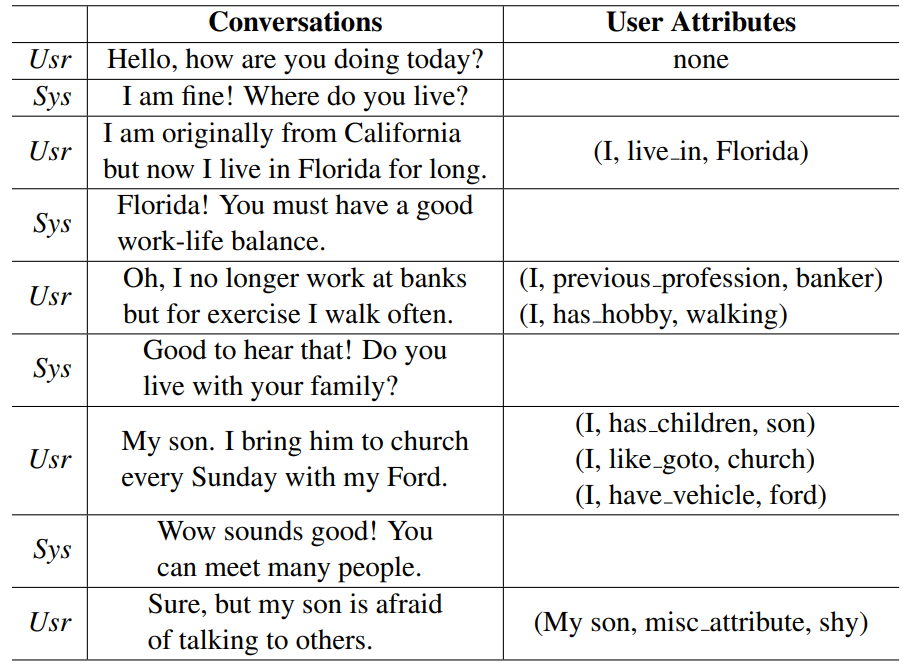
\includegraphics[width=0.8\textwidth]{images/gtky_task.png}
    \caption{Реплики и извлеченные из них кортежи. Пример взят из статьи \cite{gtky}}
    \label{fig:gtky_task}
\end{figure}

 Основную сложность в данной задаче определяет отсуствие датасета с качественной разметкой и методов обучения без учителя.
 

        \newpage 
	\chapter{\centering\normalsize{ОСНОВНАЯ ЧАСТЬ}}
\addcontentsline{toc}{section}{ОСНОВНАЯ ЧАСТЬ}

\section{Релевантные исследования}
К представленному в данной работе исследованию имеются несколько смежных задач и направлений. Ниже описан краткий обзор по каждому направлению и существующих подходов решения поставленных там задач.

\textbf{Извлечение персональных атрибутов}  Большинство работ по извлечению персональных характеристик из естественного языка использовали технику distant supervision и эвристические методы и шаблоны (\cite{pappu-rudnicky-2014-knowledge}, \cite{tigunova_2019}, \cite{gtky}, \cite{mazare-etal-2018-training}), у которых довольно низкая полнота (recall). В исследованиях в этой работе так же используется distant supervision. Тем не менее, он не критичен для работоспособности framework'a и служит исключительно как способ оценить качество представленных подходов и сравнить их с другими методами. В \cite{personachat} представлен датасет, состоящий из повседневных диалогов с описаниями персон каждого собеседника из 5-6 предложений, и ставится задача генерации ответа по входному контексту диалога используя персону собеседника и собственную персону. Тем не менее, выделение релевантных частей персоны к определенной реплике не является основным фокусом исследования. Аналогичная работа была проделана в статье \cite{focus}: в описанной архитектуре модели используется компонента retrieve'a нужного участка персоны, которая наиболее релевантна к текущему контексту диалога. Тем не менее, эти работы не ориентируются непосредственно извлекать эти атрибуты из диалогов, а использовать их в генерации ответа неявным образом. Наиболее близкими исследованиями к данной работе являются \cite{gtky} и \cite{genre}. В \cite{gtky} представляется архитектура модели состоящая из двух компонент: классификатор отношений и генератор сущностей, и обе обучаются в сквозном режиме как одно целое. В одном из подходов решения задачи в данной работе так же было решено придерживаться этой архитектуры, однако позже будет показано, что эти компоненты могут быть не связаны друг с другом для достижения хорошего качества. Стоит так же отметить, что в отличие от этого подхода, подход представленный в данной работе использует модели основанные на трансформер \cite{vaswani2017}, что заметно улучшает качество. Другой подход, описанный в \cite{genre} так же использует две компоненты: одну для генерации триплетов, и другую - для оценки релевантности сгенерированного триплета к реплике. Задачу извлечения признаков авторы \cite{genre} разделяют на две подзадачи: на явное извлечение атрибутов - когда некоторое отношение является подстрокой в реплике, и неявное - когда отношения нужно выводить из реплики основываясь на семантику. Хотя подход показал себя хорошо в указанных подзадачах, в общем случае, неизвестно под какую из этих подзадач подходит входная реплика.

\textbf{Построение графов знаний}   Установленный формат в котором извлекается информация в данной работе очень похож на структуру графов знаний, в которых граф так же хранится в виде кортежей из трех элементов: две сущности, и отношение между ними. В данной работе, кортежи извлекаются с помощью языковых моделей, включая авторегрессионные, которые были использованы в заполнении графов знаний (\cite{bosselut-etal-2019-comet}). В \cite{alt2019improving} использовалась модель GPT \cite{gpt2} для классификации отношения по заданным двум сущностям. Тем не менее, в данной работе авторегрессионная модель работает в обратном режиме, то есть по заданной реплике и отношению, она генерирует две сущности находящиеся в реплике в данном отношении.

\textbf{Извлечение информации}  В обработке естественного языка очень важны и хорошо изучены подходы извлечения информации в открытой и закрытой форме (\cite{banko2007}, \cite{wu-weld-2010-open}, \cite{berant-etal-2011-global}, \cite{fader2014}). Научным сообществом были представлены методы основанные, и на шаблонах (\cite{mausam-etal-2012-open}, \cite{delcorro2013}), и на обучаемых моделях (\cite{zeng-etal-2014-relation}, \cite{xu-etal-2015-classifying}, \cite{stanovsky-etal-2018-supervised}, \cite{vashishth-etal-2018-reside}), однако большинство из этих подходов извлекают информацию путем проставления тегов на части предложения. Дополнительно можно считать, что задача поставленная в этой работе относится к семейству задач отслеживания состояния диалога (dialogue state tracking \cite{dstc_survey}).

        \newpage
        \section{Данные}
Датасета для обучения моделей для извлечения атрибутов пока не существует. Из-за этого, в данной работе взаимствован датасет GTKY из статьи \cite{gtky}. Он создан методом distant supervision из датасета DialogueNLI \cite{dnli}, который в свою очередь построен на основе датасета PersonaChat \cite{personachat}. Ниже будет дан краткий обзор каждого из датасетов.

\textbf{PersonaChat}    Датасет содержащий примерно 10.000 диалогов открытого домена, в среднем состоящие из 10-15 реплик. Имеется разметкая каждого диалога по персонам собеседников. Пример диалога можно увидеть на Рисунке \ref{fig:pc_sample}. В датасете насчитывается 1155 персон с 5000 предложениями в неструктурированном формате на естественном языке, которые идут перед диалогами, но при этом, нет четкого соответствия между предложениями персоны и репликами.

\textbf{DialogueNLI}    Относительно новый датасет для NLI задач (\cite{nli_survey}) в диалоговом домене, построенный над датасетом PersonaChat. Состоит из пар реплик с метками импликации, нейтральности и противоречия (entailment, neutral, contradiction). Например, на Рисунке \ref{fig:pc_sample} реплика Персоны А "I just got back from the club." является следствием предложения "I like to dance at the club.". Каждое предложение персоны в датасете имеет разметку в виде триплета \textit{(subject, relation, object)}, в котором \textit{relation} - это отношение из предопределенного множества отношений, например \textit{live\textunderscore in\textunderscore general}, \textit{like\textunderscore goto}, \textit{have\textunderscore pet}. В датасете DialogueNLI таких отношений 61, и все множество этих отношений можно найти в приложениях к статье \cite{dnli}. C примерной структурой датасета можно ознакомиться на Рисунке \ref{fig:dnli_sample}.

\textbf{GTKY}   Так как в датасете DialogueNLI не все реплики имеют разметку по триплетам, авторы статьи \cite{gtky} применили SOTA NLI модель, чтобы соотнести предложения персон к репликам. То есть, если предложение персоны и реплика имеют положительный entailment, то какой то атрибут из этой реплики представляется в виде триплета соответствующего этому предложению персоны. Например, реплика "I prefer basketbal; team sports are fun." и предложение "I like playing basketball." имеют положительный entailment, поэтому данной реплике можно присвоить триплет персоны \textit{(I, like\textunderscore sports, basketball)} в качестве одного из атрибутов. В качестве NLI модели для определения степени entailment'a двух предложений был использован BERT \cite{devlin_bert}, дообученный на датасете DialogueNLI, который получил точность 88.43\% на тестовой выборке.

\subsection{Анализ датасета GTKY}

Размеры обучающей, тестовой и валидационной выборки равны 131.424, 15.008 и 15.586 соответственно. Cо статистиками по распределению количества триплетов по репликам можно ознакомиться в Таблице \ref{table:triple_count_stats} и на Рисунке \ref{fig:triple_distr}. Как можно увидеть, в датасете около 50\% примеров имеют пустой целевой набор атрибутов. Так же можно посмотреть на распределение типов отношений на Рисунке \ref{fig:predicate_distr}, а самые часто и самые редко встречающиеся сущности показаны в Таблице \ref{table:top5_subj} и \ref{table:top5_obj}.

Техника distant supervision заменяет человеческую разметку данных, однако, вводит другие трудности, представленные шумом в данных что видно в Таблице \ref{table:gtky_noise}.
 
\begin{figure}[!ht]
    \centering
    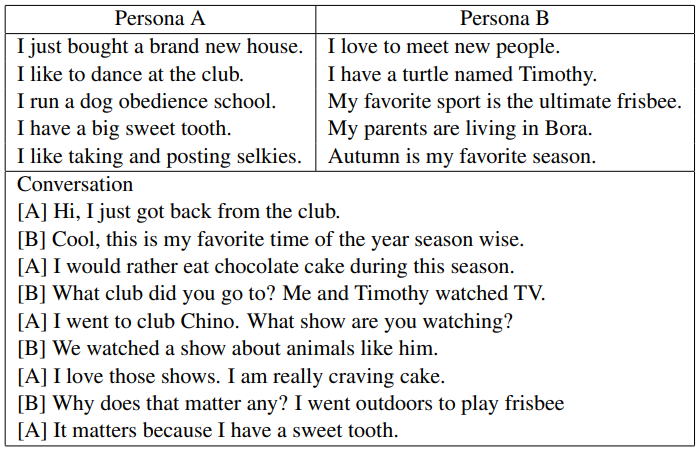
\includegraphics[width=0.8\textwidth]{images/pc_example.png}
    \caption{Пример диалога из датасета PersonaChat. Персоны собеседников заданы перед диалогом.}
    \label{fig:pc_sample}
\end{figure}

\begin{figure}[!ht]
    \centering
    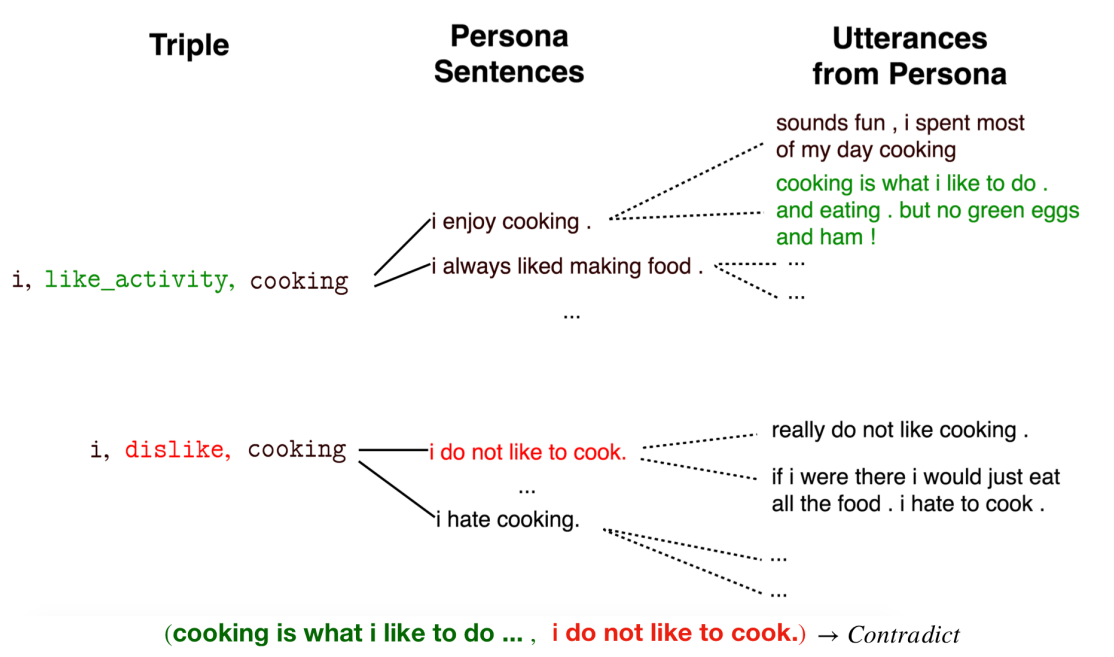
\includegraphics[width=0.8\textwidth]{images/dnli_example.png}
    \caption{Пример из датасета DialogueNLI и схема соотношения триплетов к репликам.}
    \label{fig:dnli_sample}
\end{figure}

\begin{table}[!ht]
\centering
\begin{tabular}{c|c c c}
    \hline
     & TRAIN & TEST & VALIDATION \\
    \hline
    \hline
    \textbf{max} & 6 & 5 & 5 \\
    \hline
    \textbf{mean} & 0.61 & 0.61 & 0.63 \\
    \hline
    \textbf{median} & 0 & 0 & 1 \\
    \hline
\end{tabular}
\caption{Статистики количества триплетов в репликах в датасете GTKY.}
\label{table:triple_count_stats}
\end{table}

\begin{figure}[!ht]
    \centering
    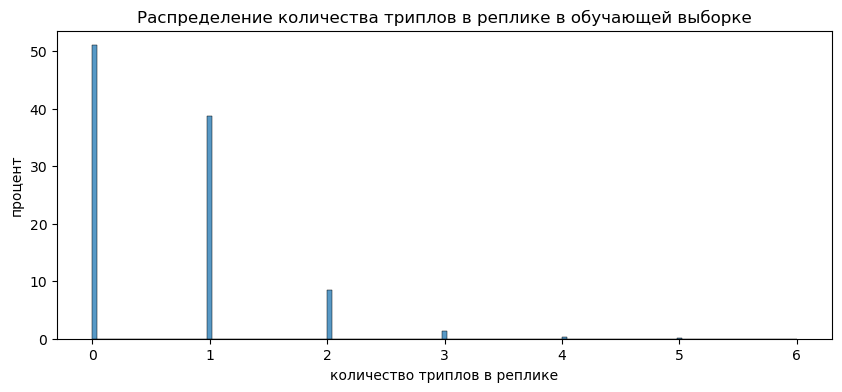
\includegraphics[width=0.9\textwidth]{images/triple_distr_train.png}
    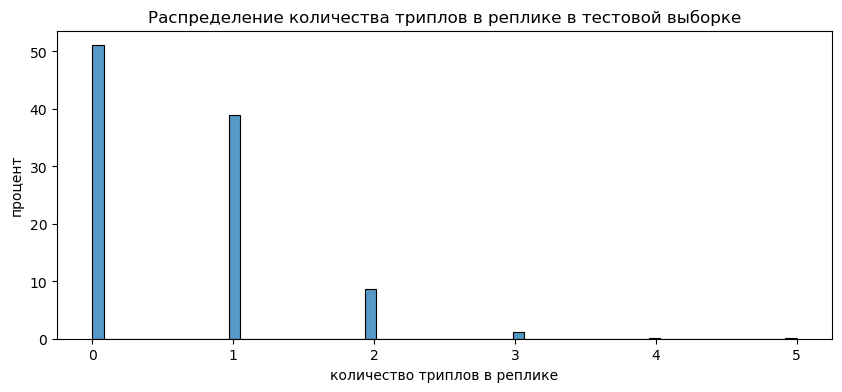
\includegraphics[width=0.9\textwidth]{images/triple_distr_test.png}
    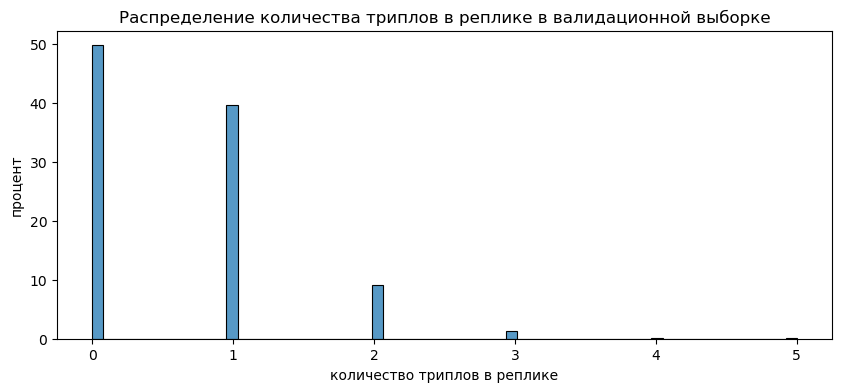
\includegraphics[width=0.9\textwidth]{images/triple_distr_val.png}
    \caption{Распределения количества триплетов в репликах в разных выборках датасета GTKY.}
    \label{fig:triple_distr}
\end{figure}

\begin{figure}[!ht]
    \centering
    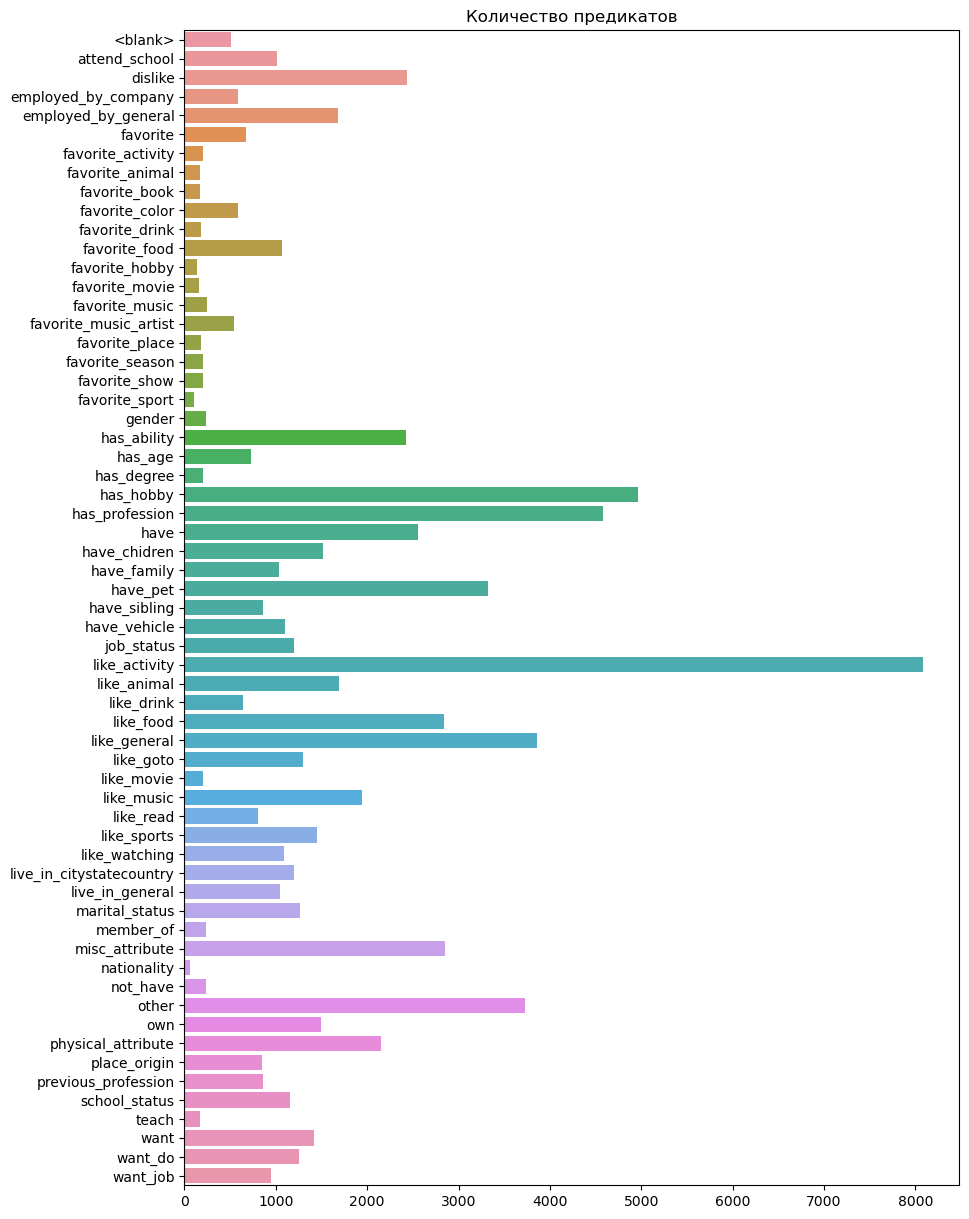
\includegraphics[width=0.95\textwidth]{images/predicate_distr.png}
    \caption{Распределение типов отношений в обучающей выборке датасета GTKY.}
    \label{fig:predicate_distr}
\end{figure}

\begin{table}[!ht]
\centering
\begin{tabular}{|c|c|}
    \hline
     Субъект & Количество \\
     \hline
    i & 75202 \\
    \hline
    my mother & 988 \\
    \hline
    my & 567 \\
    \hline
    my brother & 204 \\
    \hline
    my parents & 203 \\
    \hline
    \hline
    my career & 1 \\
    \hline
    my marriage & 1 \\
    \hline
    commitment & 1 \\
    \hline
    my foster & 1 \\
    \hline
    dude & 1 \\
    \hline
\end{tabular}
\caption{Топ-5 самых часто и редко встречаемых субъектов среди триплетов в обучающей выборке датасета GTKY.}
\label{table:top5_subj}
\end{table}

\begin{table}[!ht]
\centering
\begin{tabular}{|c|c|}
    \hline
     Объект & Количество \\
     \hline
    dog & 1530 \\
    \hline
    \texttt{<blank>} & 1336 \\
    \hline
    cat & 992 \\
    \hline
    student & 760 \\
    \hline
    cooking & 723 \\
    \hline
    \hline
    hard time & 1 \\
    \hline
    5 pets & 1 \\
    \hline
    carriage & 1 \\
    \hline
    group & 1 \\
    \hline
    significant other & 1 \\
    \hline
\end{tabular}
\caption{Топ-5 самых часто и редко встречаемых объектов среди триплетов в обучающей выборке датасета GTKY.}
\label{table:top5_obj}
\end{table}

\begin{table}[!ht]
% \centering
\begin{tabular}{|m{15em}|m{15em}|}
    \hline
     Реплика & триплет \\
     \hline
     \hline
    all i can think about is moving away. & \textit{(my, like\textunderscore goto, desert)} \\
    \hline
    i have a wife i am in my early 40s. & \textit{()} \\
    \hline
    she is a golden retriever very nice dogs. & \textit{(my dog, other, name wonwon)} \\
    \hline
    i like to meet new people. & \textit{(i, live\textunderscore in\textunderscore citystatecountry, new york)} \\
    \hline
    i already mentioned them. but i like to spend time with my family and dogs. & \textit{()} \\
    \hline
    do you work anywhere ? i have a part time job. & \textit{()} \\
    \hline
    sounds like some awesome films. & \textit{(i, like\textunderscore goto, movie theater)} \\
    \hline
    rather get to know you i got free hp computer today. & \textit{(my adopted father, employed\textunderscore by\textunderscore company, hp)} \\
    \hline
\end{tabular}
\caption{Шум в разметке датасета GTKY с distant supervision.}
\label{table:gtky_noise}
\end{table}

        \newpage
        \section{Методология}
Для решения поставленной задачи предлагаются два основных подхода: прямой sequence-to-sequence подход (GenAE) и двухэтапный метод (PipelineAE). В данном разделе описываются эти подходы и их достоинства с недостатками.

\subsection{GenAE}\label{sbs:direct_method}
C общей архитектурой этого метода можно ознакомиться на Рисунке \ref{fig:mt5_arch}. В данном подходе используется sequence-to-sequence модель для генерации набора триплетов непосредственно из реплики. То есть решается задача языкового моделирования \cite{bengio_nlm}:
\begin{equation}\label{lm_loss}
    \log P(y_i | y_{i-1}, ..., y_0, \mathbf{X}) \rightarrow \max,
\end{equation}
где $y_i$ - это:
\begin{itemize}
    \item правильный следующий токен из словаря модели;
    \item токен \texttt{<subj>} - специальный токен, после которого должен сгенерироваться субъект в триплете;
    \item токен \texttt{<rel>} - специальный токен, после которого должно сгенерироваться отношение в триплете;
    \item токен \texttt{<obj>} - специальный токен, после которого должен сгенерироваться объект в триплете;
    \item токен \texttt{<none>} - специальный токен, который означает, что реплика не содержит триплетов;
\end{itemize}
и $\mathbf{Y}=(y_0,...,y_i,...,y_n)$ - это набор триплетов разеделнных знаком ";" либо "\texttt{<none>}", а $\mathbf{X}$ - это входная реплика. То есть модель обучается на максимизации логарифма вероятности следующего токена учитывая контекст и вход. Следует заметить, что подходит и обычная генеративная модель, то есть нет преимущества использовать обязательно encoder-decoder модели. Но в экспериментах в данной работе были использованы mT5 в base и small размерах, которые имеют архитектуру encoder-decoder.

Например, по реплике "My brother likes to eat plov." модель должна сгенерировать "\texttt{<subj> I <rel> have\textunderscore sibling <obj> brother; <subj> my brother <rel> like\textunderscore food <obj> plov}", а по реплике "Hello, how are you doing today?" - "\texttt{<none>}".

Основным преимуществом GenAE является то, что он прост в реализации и хорошо работает в случаях, когда реплики короткие и содержат не более одного триплета. Так как в остальных случаях, для лучшего качества требуется соблюсти порядок триплетов в котором они встречаются во входной реплике. Важно так же заметить, что результаты модели плохо интерпретируемы, так как нет возможности узнать уверенность модели в выборе определенного отношения из общего множества. Брать уверенность модели в сгенерированных токенах отношения во время генерации некорректно из-за того, что вероятность в таком случае вычисляется не по множеству отношений, а по множество всех токенов в словаре модели. Другой недостаток модели в том, что генеративные модели не предобучаются извлекать структурированную информацию из входного текста, и применение их в подобных задачах может показать низкие результаты, если неправильно аугментировать их способности. Например, в данной задаче на одну модель накладывается несколько подзадач одновременно: определение релевантных отношений в реплике и генерация сущностей. Это может помешать модели выделять сразу несколько триплетов из реплик, что и наблюдалось в экспериментах.

\begin{figure}[!ht]
    \centering
    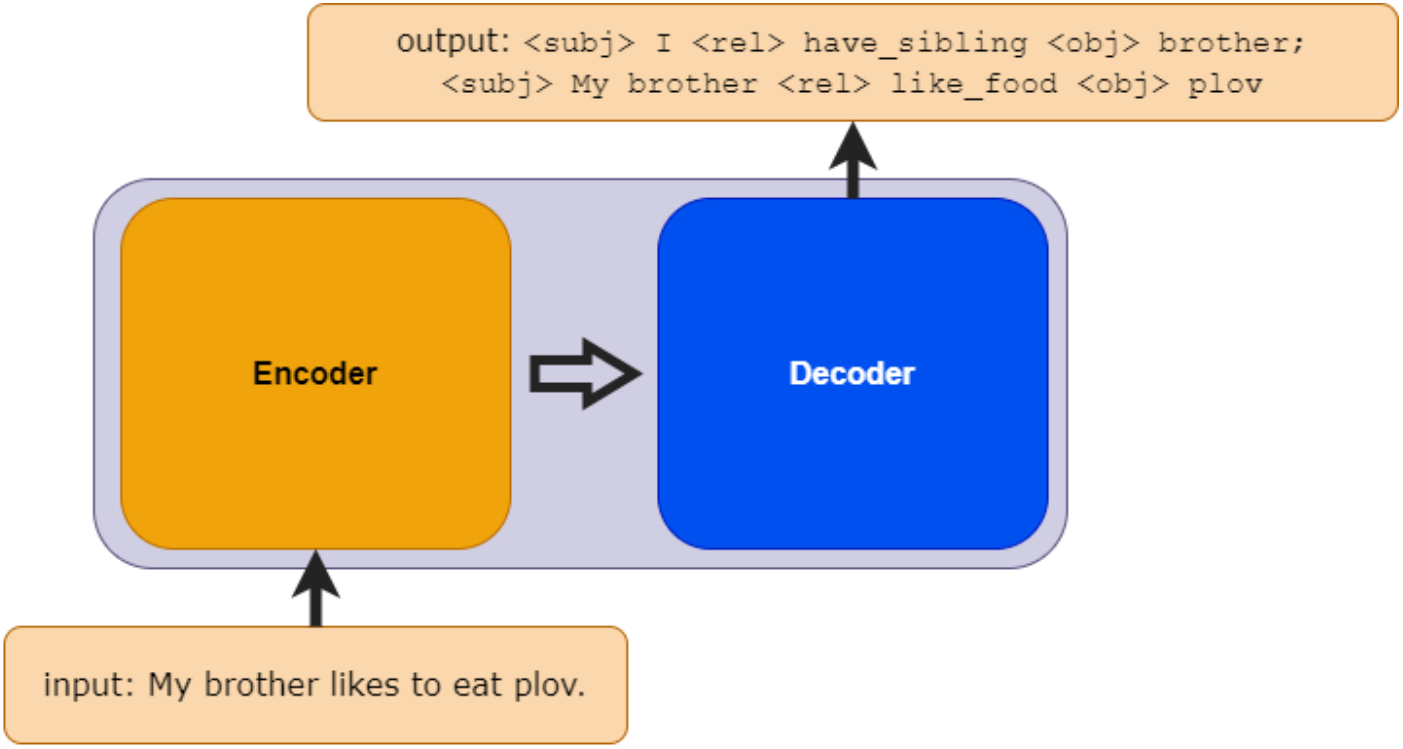
\includegraphics[width=0.8\textwidth]{images/mt5_arch.png}
    \caption{Общая архитектура решения прямым методом используя seq2seq модель.}
    \label{fig:mt5_arch}
\end{figure}

\subsection{PipelineAE}
Общая архитектура данного подхода изображена на Рисунке \ref{fig:full_arch}. В нем поставленная задача делится на две очевидные подзадачи: выявление существующих в реплике отношений и по этим отношениям и реплике генерация сущностей: субъектов и объектов. Ниже будут описаны модели и методы, которые решают эти подзадачи. Из достоинств PipelineAE можно выделить интерпретируемость результатов и расширяемость, так как, как можно будет узнать позже, большинство методов решения этих подзадач применимы в few-shot подходах. Так же модели обучаются одновременно благодаря тому, что данные на которых они обучаются независимы. Из недостатков можно отметить увеличенный объем вычислений и моделей, что может затруднять поддержку этих моделей в индустриальном применении.

\begin{figure}[!ht]
    \centering
    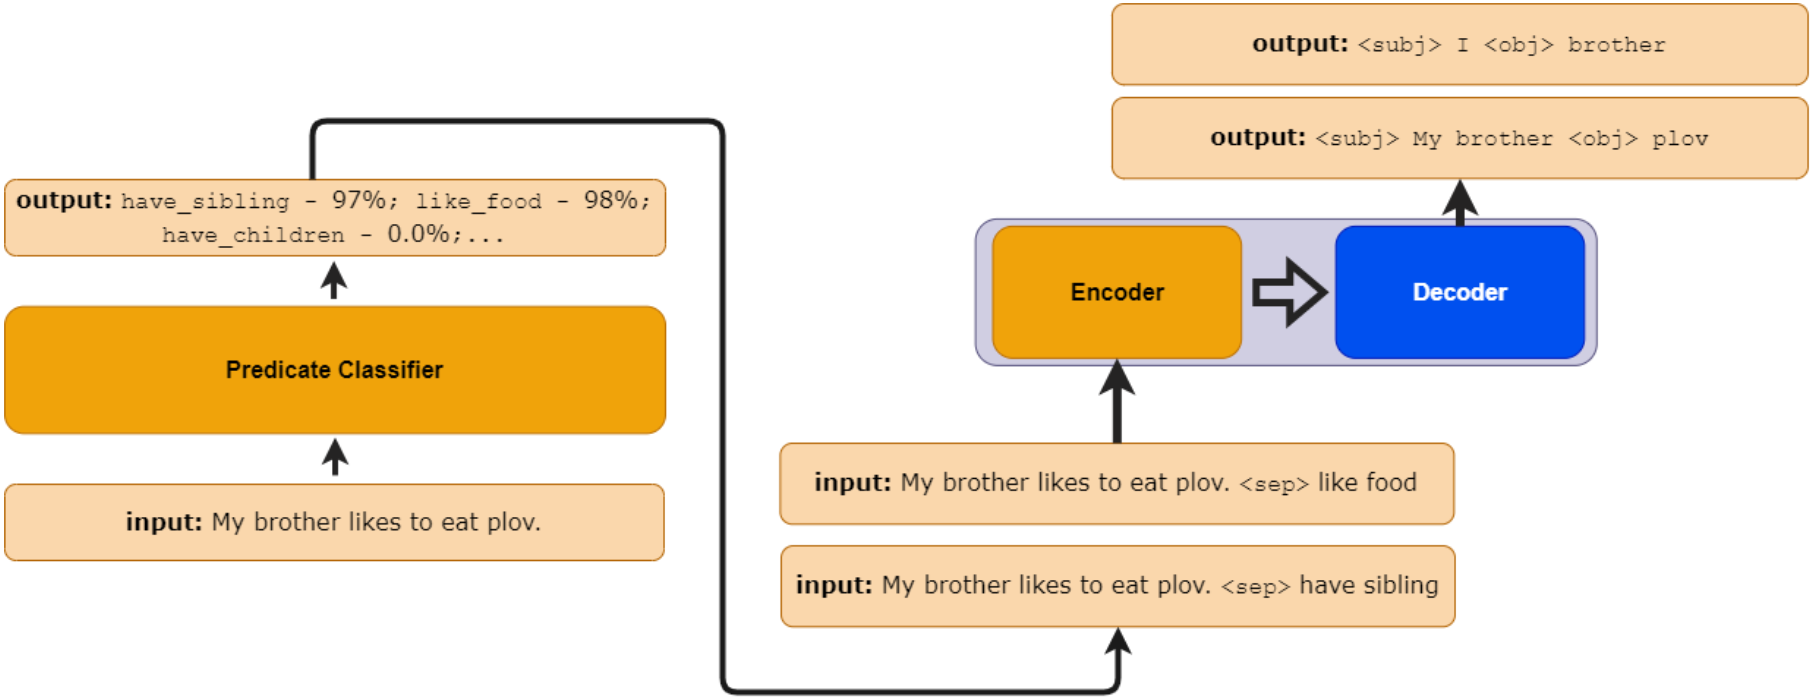
\includegraphics[width=1.0\textwidth]{images/full_arch.png}
    \caption{Общая архитектура PipelineAE. Реплика сначала подается на вход классификатору предикатов (слева) и по выделенным предикатам и реплике генерируются сущности (справа).}
    \label{fig:full_arch}
\end{figure}

\subsubsection{Классификатор предикатов}
Задачу выявления отношений из реплик можно сформулировать как multi-label classification, то есть по входной реплике предсказывается множество отношений которые присутствуют в ней, как на Рисунке \ref{fig:pred_cls}. Стоит заметить, что множество может быть и пустым.

\begin{figure}[!ht]
    \centering
    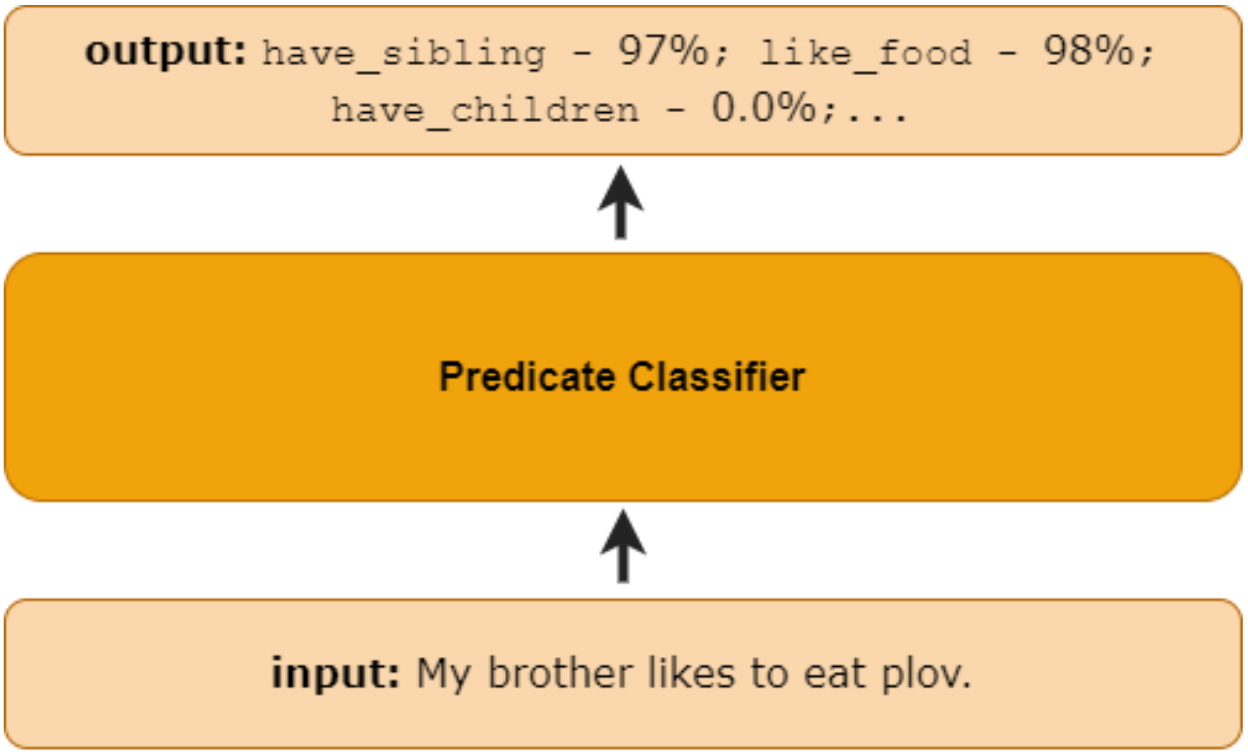
\includegraphics[width=0.8\textwidth]{images/pred_cls.png}
    \caption{Классификатор предикатов по входной реплике. Результат представляется в режиме multi-label classification.}
    \label{fig:pred_cls}
\end{figure}

\textbf{Multi-label classification} Можно решать задачу напрямую и в таком случае телом классификатора может служить любая SOTA BERT-подобная модель для текстовой классификации, эмбеддинг токена \texttt{[CLS]} которой в последнем слое проходит через линейный слой и активацию vector-wise sigmoid:

\begin{equation}\label{sigmoid}
    Sigmoid(x) = \frac{1}{1 + e^{-x}}
\end{equation}

В качестве функции потерь тут служит binary cross-entropy loss:

\begin{equation}\label{bce_loss}
    L(x,y) = \frac{1}{C} \sum^{C}_{i=1}{l_i(x, y)},
\end{equation}

где $C$ - количество классов, в данном случае количество предопределенных отношений $|R|$, 

\begin{equation}\label{relation_set}
    R=\{r_1,...,r_C\}
\end{equation}

, $x$ - logit'ы модели по входной реплике, 

\begin{equation}\label{target_indicator}
    y = ([r_1 \in Y], [r_2 \in Y], ..., [r_C \in Y])^\mathsf{T}
\end{equation}

, $Y$ - множество отношений в реплике, a

\begin{equation}\label{bce_loss_component}
    l_i(x, y) = -[w_i \cdotp y_i \cdotp \log{p_i} + (1 - y_i) \cdotp \log{(1 - p_i)}],
\end{equation}

где $p_i = Sigmoid(x_i)$. В формуле \ref{bce_loss_component} можно увидеть $w_i$ - вес присутсвия $i$-го предиката в целевом множестве отношений по данному входу. Например, если в датасете у 100 реплик есть этот предикат в целевых наборах предикатов, а у 300 его нет, то $w_i = \frac{300}{100} = 3$, что значит, что для модели в датасете не будет дизбаланса классов, что полезно в случаях multi-label classification когда датасет всегда дизбалансный, если рассматривать маргинальные распределения каждого предиката по отдельности. Этот метод широко известен под названием binary-relevance \cite{binary_relevance} и в нем каждый класс рассматривается независимо от других, что не всегда может быть правильно в некоторых задачах, если классы имеют некоторую иерархическую онтологию.

\textbf{Binary ranking} В таком подходе ставится задача определения релевантности отношения к реплике, то есть по входной реплике и описанию предиката ставится задача бинарной классификации. В качестве модели можно снова брать любую SOTA BERT-подобную модель для классификации пар текстов. Можно подавать вместо описания предиката сам предикат, но тогда качество будет относительно хуже, из-за небольшого количества семантической информации и присутствия токена "\_" нижнего подчеркивания в отношении, который непривычен для предобученных языковых моделей. Таким, образом, на вход модели передается строка в формате "X \texttt{[SEP]} Y", где Х - реплика, а Y - описание предиката; и на выходе модели ожидается вероятность того, находится ли предикат соответствующий описанию Y в реплике Х. Для такого подхода датасет преобразовывается следующим образом: 
\begin{enumerate}
    \item рассматривается каждый пример из исходного датасета GTKY;
    \item если у реплики непустой целевой набор атрибутов, то для каждого отношения из этого набора формируется "положительная" пара "X \texttt{[SEP]} Y" и добавляется в новый датасет, а из дополнения этого набора от общего множества случайным образом добирается N отношений чтобы сформировать "отрицательные" пары. Таким образом, каждой положительной паре соответствует N отрицательных пар;
    \item если у реплики пустой целевой набор атрибутов, то к этой реплике из множества всех отношений добирается N / 2 отношений для формирования отрицательных пар и добавляется в новый датасет. Эвристика деления N на 2 помогает избавиться от чрезмерного увеличения отрицательных примеров в новом датасете, так как, как можно было увидеть ранее, исходный датасет содержит очень много реплик без каких-либо атрибутов.
\end{enumerate}
Этот подход называется negative sampling и часто используется для обучения моделей retrieve'a документов или в построении графов знаний. От параметра N зависит размер полученного датасета и отношение положительных и отрицательных примеров. Если N слишком большой, то будет смещение в сторону отрицательного класса, а если N слишком маленький, то модель не научится различать все пары реплик и предикатов. В экспериментах были рассмотрены N=4 и N=9, и было замечено что N=4 дает более приемлимый результат. Важно так же заметить, что при отборе неподходящих отношений нужно рассматривать их равновероятно и с разными seed'ами, чтобы в полученном датасете каждый тип отношений встречался примерно одинаковое количество раз, тогда модель сможет увидеть все отношения из множества и оценить их релевантность к репликам. В качестве функции потерь берется аналогичная \ref{bce_loss_component} функция, однако не учитывается вес положительных примеров, так как баланс классов контролируется параметром N.

Для предсказания по входной реплике Х набора отношений с помощью такой модели, в нее подается каждая пара "X \texttt{[SEP]} $desc(r_i)$" $\forall r_i \in R$ и получаются оценки релевантности, и оставляются только те отношения, для которых оценка выше определенного порога. Очевидно, таким образом, сложность процесса предсказания модели равна $O(M \cdotp C)$, где $M$ - количество реплик в тестовой выборке и $C$ - количество отношений, в то время как у предыдущего подхода она равна $O(M)$. Это основной недостаток данного подхода, однако это дает ему возможность легко обобщаться на новые предикаты, благодаря рассмотрению их описаний на естественном языке.

\textbf{Contrastive learning}   В этом подходе также используется negative sampling: для каждой реплики и каждого положительного предиката добирается по N отрицательных предикатов. Для случаев, когда реплика не имеет предикатов, дополнительно вводится предикат \texttt{<none>} и добавляется в множество отношений, то есть он может быть отобран в
процессе negative sampling.

После вышеуказанного преобразования исходного датасета, можно предположить, что получится датасет:

\begin{equation}\label{nll_dataset}
    \mathcal{D} = \{(q_i, r^{+}_{i}, r^{-}_{i, 1},..,r^{-}_{i, N})\}_{i=1}^{M},
\end{equation}

который состоит из $M$ примеров, каждый из которых содержит реплику $q_i$ , один релевантный (положительный) предикат $r^{+}_i$ и N отрицательных предикатов. Во время обучения минимизируется отрицание логарифма правдоподобия положительного предиката:

\begin{equation}\label{contrastive_loss}
    L(q_i, r^{+}_{i}, r^{-}_{i, 1},..,r^{-}_{i, N}) =
    -\log{\frac{e^{sim(q_i, r^{+}_i)}}{e^{sim(q_i, r^{+}_i)} + \sum^{N}_{j=1}{e^{sim(q_i, r^{i}_{i, j})}}}},
\end{equation}

где,

\begin{equation}\label{similarity_func}
    sim(q, r) = BERT("q \texttt{[SEP]} desc(r)"),
\end{equation}

то есть используется архитектура BERT-подобной модели для задачи регрессии, эмбеддинг токена \texttt{[CLS]} который проходит через полносвязный слой который на выходе дает одно вещественное число - similarity. Такой подход был использован в dense passage retrieval \cite{dpr} и показал хороший результат.

В таком подходе, N также является важным параметром, и чем он больше, тем лучше модель учится оценивать правдоподобие релевантного предиката, но это увеличивает количество вычислений в N раз, и во время обучения произойдет $O(M \cdotp N)$ forward вызовов у модели, что конечно является основным недостатком данного подхода. Тем не менее, этот подход так же легко обобщается на новые предикаты, и часто применяется для few-shot классификации.

Предсказания можно получить аналогично предыдущему подходу, только теперь модель на выходе дает не вероятности, а неограниченные вещественнозначные числа - similarity между репликой и описанием предиката на естественном языке. Это может стать проблемой при выборе порога выбора ответа, так как сложно оценить диапазон значений, но эту проблему можно устранить функцией активации которая сжимает значения схожести в определенном отрезке, но это может вызвать проблему затухающих градиентов.

\subsubsection{Генератор сущностей}

После определения всех предикатов в реплике, ставится задача генерации сущностей по заданной реплике и отношению, которые находятся в данном отношении. Можно свести данную задачу к задаче заполнения недостающих частей текста (\textit{span corruption}) чем хорошо справляются современные sequence-to-sequence модели. Задачу можно продемонстрировать на Рисунке \ref{fig:egen}, либо таким примером:

\begin{verbatim}
utt = i have two boys and they are always hungry.
rel = have children
input:
{utt} <sep> <subj> <span_1> <rel> {rel} <obj> <span_2> 
output:
<span_1> i <span_2> 2 son
\end{verbatim}
, где \texttt{<span\textunderscore 1>} и \texttt{<span\textunderscore 2>} обозначают пропуски в тексте. В данном случае пропусков всегда два: это субъект и объект триплета которые нужно сгенерировать. По сути, задача такая же как в GenAE \ref{sbs:direct_method}, и оптимизируется такая же функция потерь как в \ref{lm_loss}, но вход в модель теперь содержит и существующее отношение в реплике. Важно заметить, что модель в таком подходе обучается генерировать сущности только по отношению которое присутствует в реплике, и если подавать отсутствующий в реплике предикат, поведение модели неопределено.

\begin{figure}[!ht]
    \centering
    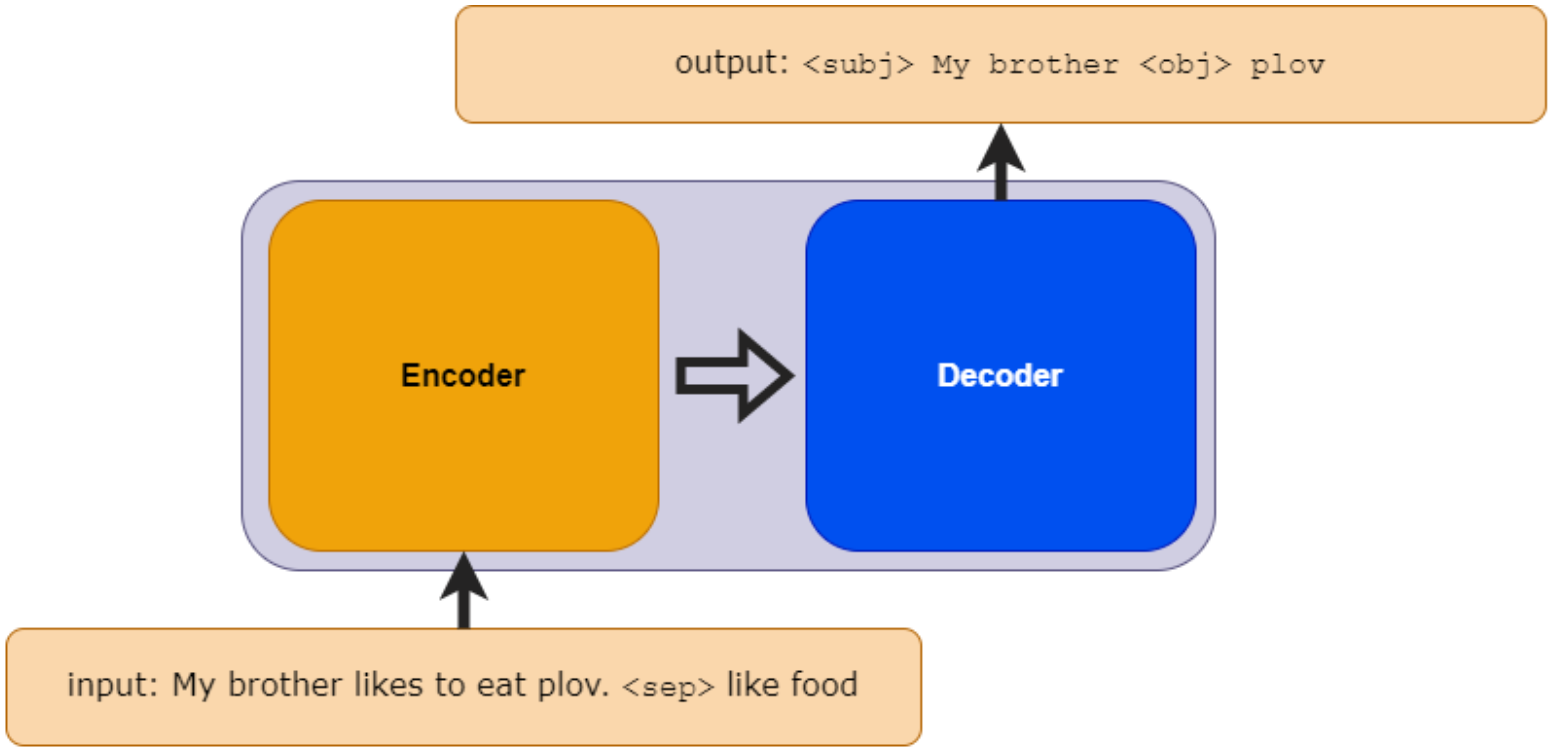
\includegraphics[width=0.8\textwidth]{images/egen.png}
    \caption{Генератор сущностей использующий seq2seq модель. Принимает на вход пару: реплика и предикат, который присутствует в данной реплике, и генерирует субъект и объект находящиеся в соответствующем отношении в реплике.}
    \label{fig:egen}
\end{figure}

        \newpage
        \section{Эксперименты}

В данном разделе описаны детали экспериментов проведенных используя вышеописанную методологию и метрики качества вместе с базовыми моделями. Тут важно отметить, что в экспериментах были использованы многоязычные версии популярных трансформеров, чтобы их можно было дообучить с небольшим количеством данных на целевом языке и получить рабочие модели на этом языке.

\subsection{Детали обучения}
Все модели обучались на двух видеокартах NVIDIA A100 40gb. В качестве оптимизатора был использован AdamW \cite{adamw} c \texttt{weight\textunderscore decay=0.01}. Шаги обучения и размеры batch'a варьировались в зависимости от модели. Ниже описаны детали по каждому подходу (размеры batch'a указаны для каждого вычислительного устройства):

\textbf{GenAE}   В качестве sequence-to-sequence моделей были выбраны mT5-small и mT5-base \cite{mt5}. Шаг обучения для обеих моделей был равен 0.0003, а размер batch'a для базового варианта модели 32, а для маленького варианта - 64. Обучение длилось 3 эпохи с классом \texttt{Seq2SeqTrainer} библиотеки Huggingface Transformers \cite{wolf2019hf}. Генерация происходит жадным декодированием, то есть в качестве следующего токена всегда выбирается токен с наибольшей условной вероятностью.

\textbf{Классификатор предикатов}   В качестве базовой архитектуры BERT-подобной модели для текстовой классификации были выбраны многоязычный DistilledBERT \cite{distilbert} и mBERT-base. Для multilabel classification были подобраны веса положительных классов как описано в формуле \ref{bce_loss_component} в одном эксперименте, и в другом - приравнивались 1. Шаг обучения для всех экспериментов с этой моделью был равен 0.00003, а для binary ranking и contrastive learning 0.00002. Размер batch'а для multilabel classification был равен 512, для contrastive learning - 10, для binary ranking - 128. Для binary ranking были так же рассмотрены mBERT-base и mDeBERTa-NLI base. NLI модель рассматривалась для улучшения качества определения релевантности предиката. Изначально, в экспериментах предикаты подавались на вход моделям как есть, позже было решено использовать их описания на естественном языке, что везде улучшило качество. Во всех подходах модели обучались в течение 5 эпох, кроме contrastive learning в котором обучение длилось 4 эпохи.

Процессы получения предсказаний у подходов binary ranking и contrastive learning очень похожи, то есть обе модели принимают на вход пару реплики и описания предиката и дают на выходе число, либо вероятность релевантности предиката, либо схожесть описания предиката и реплики, и для корректности предсказаний требуют установления определенного порога. Порог можно подобрать жадным образом. Для простоты, в данной работе порог был подобран для всех предикатов один в обоих подходах. Это также связано с предположением, что в данных подходах модели не совсем ограничены предопределенным множеством предикатов и обучаются на описаниях отношений на естественном языке, а не на самих предикатах, для достижения обобщающей способности. Таким образом:

\begin{enumerate}
    \item для binary ranking выбирается равномерная сетка в отрезке $[0, 1]$ и считается multi-label micro-averaged F1 на валидационной выборке и выбирается порог с наибольшим показателем данной метрики;
    \item для constrastive learning действуем аналогично пункту 1, но равномерная сетка строится на отрезке $[\min, \max]$, где $\min$ - минимальное значение схожести на валидационной выборке, а $\max$ - соответственно наибольшее;
    \item если же в contrastive learning модель на выходе дает числа из специфичного диапазона, например из $[-1, 1]$ или $[0, 1]$ поступаем аналогично пункту 1.
\end{enumerate}

\textbf{Генератор сущностей}    Для этого подхода был использован mT5-small. В качестве оптимизатора был изначально выбран AdaFactor \cite{adafactor}, с помощью которого все Т5 модели были предобучены, однако независимо от размера шага, с этим оптимизатором генератор сущностей переобучался начиная уже с ранних этапов обучения. Из-за этого по итогу было решено обучать только оптимизатором AdamW с \texttt{lr=0.00005} с размером batch'a 64. Дополнительно, для ускорения обучения модель была обучена в mixed-precision режиме с float16, но по итогу эксперимента во всех случаях было переполнение в представлении вещественных чисел float16. В каждом подходе модели обучались в течение 5 эпох. Генерация как и в GenAE, происходит жадным декодированием.

\textbf{Метрики качества}   Чтобы оценить итоговое качество извлечения триплетов из реплик берутся accuracy, F1 и BLEU-1. Accuracy и F1 считаются по точному совпадению полученных триплетов: recall равен отношению количества правильно сгенерированных триплетов на количество всех триплетов в тестовой выборке, а precision - это отношение количества правильно сгенерированных триплетов к количеству всех сгенерированных триплетов. В то время, как BLEU-1 более гибкий и учитывает нестрогое совпадение между триплетами. 
Для оценки качества классификатора предикатов применялись accuracy и multi-label F1. А генератор сущности оценивался в конечном режиме, когда в качестве извлеченных предикатов подавались правильные отношения из датасета.

\textbf{GenAE на WikiNRE}   Для оценки качества sequence-to-sequence подхода был проведен дополнительный эксперимент на датасете WikiNRE \cite{trisedya-etal-2019-neural}. Детали эксперимента и результаты описаны в Приложении \ref{AppendixA}.


        \newpage
        \section{Результаты}

В данном разделе будут описаны результаты экспериментов и сравнения разных подходов, так же сделаны некоторые выводы. Все показатели моделей представленных в данной работе отобраны из лучших checkpoint'ов. Стоит отметить, что показатели даны в качестве справки, так как в данном исследовании основной целью было построить рабочий framework и протестировать его на доступном датасете. Так как сам датасет очень шумный из-за разметки с использованием distant supervision, результаты моделей недостаточно высоки.

\subsection{Базовая модель}   В качестве лучшего существующего подхода для извлечения атрибутов из реплик была выбрана модель GKTY представленная в статье \cite{gtky}. Она выбрана в качестве базовой модели, так как из всех существующих похожих подходов она решает поставленную задачу как есть, без дополнительных условностей. Модель состоит из трех компонент:

\begin{itemize}
    \item encoder входной реплики (bidirectional GRU \cite{gru}) для получения эмбеддингов;
    \item классификатор предикатов: multi-hop end-to-end memory network \cite{sukhbaatar2015} которая хорошо показала себя в задаче ответов на вопросы. Решает задачу multi-label classification;
    \item генератор сущностей (GRU \cite{gru}) который по скрытому состоянию encoder'a и предсказанному множеству предикатов генерирует соответствующие субъект и объект.
\end{itemize}

Стоит заметить, что все три компоненты этой архитектуры обучаются вместе в сквозном режиме. В PipelineAE каждая компонента может обучаться параллельно. Также можно заметить, что GenAE тоже напоминает базовую модель, так как одна архитектура решает сразу несколько задач, но все происходит неявно во время оптимизации одной функции потерь \ref{lm_loss}, в то время как у базовой модели используется взвешенная сумма разных функций потерь под каждую задачу.

\subsection{Классификатор предикатов}
В PipelineAE требуется оценить качество каждой компоненты по отдельности. В Таблице \ref{table:rel_cls_results} даны оценки качества классификации предикатов. Предсказания каждого подхода непосредственно или с некоторым преобразованием сводятся к multi-label classification, поэтому даны показатели метрик описанных в разделе экспериментов для multi-label классификации. Для binary ranking и contrastive learning даны результаты после подбора оптимального порога на валидационной выборке. Можно увидеть, что применение multi-label classification без подбора весов для положительных классов сильно смещается в сторону пустого целевого набора предикатов. Об этом говорят нулевая точность (precision) и полнота (recall), то есть модель не дает на выходе 1. Благодаря этому, accuracy этой модели равно доле реплик в датасете в которых нет предикатов вообще. После взвешивания положительных классов, получены результаты чуть лучше, но все равно это очень низко, и модель все еще смещается в сторону 0 в каждом классе. После изучения маргинальных распределений предикатов выяснилось, что и без реплик в которых нет предикатов, в датасете по каждому классу имеется доминирование 0. Тем не менее, после подбора порога получены результаты намного лучше. В случае binary ranking NLI модель показывает самые высокие результаты, уступая по F1 только классификатору предикатов в базовой модели. Тем не менее, более тщательным подбором гиперпамараметров и преобразованием данных можно получить показатели еще выше. Перенос знаних полученных в задаче NLI очевидно в данном случае помогает улучшить результат полученный моделью предобученной на MLM и next sentence prediction. было так же замечено, что из-за своего размера mDeBERTa начала переобучаться и было решено брать checkpoint на ранных стадиях обучения. В случае контрастного обучения, результат представлен у модели, которая обучалась дополнительно с активацией $Sigmoid$ на последнем слое. Хотя, независимо от того, есть сужение значений у функции или нет, модель смещается в сторону предиката "\texttt{<none>}". Чтобы бороться с этим феноменом можно не рассматривать все реплики с нулевым количеством предикатов, так как они очень часто похожи друг на друга, а выбрать среди них случайное подмножество, либо исследовать "сложные" примеры с помощью уверенности модели. Тем не менее, это исследование довольно трудоемко и оставляется на будущее. После подбора порога было замечено, что для достижения оптимального multi-label F1 у моделей в обоих подходах выбирается очень высокий порог. Для binary ranking $\approx 0.87$, а для contrastive learning с активацией $Sigmoid$ $\approx 0.98$. Возможно, это также связано с маргинальными распределениями каждого из предикатов в датасете.

\subsection{Генератор сущностей}
В Таблице \ref{table:egen_results} представлены результаты измерения качества генератора сущностей. Без особых приемов и техник кроме использования описаний предикатов вместо них самих дает достигается высокий результат. Эти показатели можно брать за потолок, который можно достичь с классификатором предикатов.

\begin{table}[!ht]
\centering
\begin{tabular}{c c c}
    & \textbf{F1} & \textbf{ACC} \\
    \hline
    \hline
    mBERT MC weighted & 14.09 & 17.11 \\
    \hline
    mBERT MC weighted (с подбором порога) & 30.03 & 41.4 \\
    \hline
    mBERT MC & 0.0 & 52.04 \\
    \hline
    DistilBERT CL & 28.38 & 26.39 \\
    \hline
    DistilBERT BR & 33.39 & 42.86 \\
    \hline
    mDeBERTa NLI BR & 38.9 & \textbf{45.64} \\
    \hline
    Базовый классификатор предикатов & \textbf{44.40} & 41.57 \\
    \hline
\end{tabular}
\caption{Результаты качества классификации предикатов. BR - binary ranking, CL -contrastive learning, MC - multi-label classification}
\label{table:rel_cls_results}
\end{table}

\begin{table}[!ht]
\centering
\begin{tabular}{c c c c}
    & \textbf{ACC} & \textbf{F1} & \textbf{BLEU-1} \\
    \hline
    \hline
    mT5-small & \textbf{70.3} & \textbf{70.6} & \textbf{96.55} \\
    \hline
    Базовый генератор сущностей & 43.48 & 46.03 & - \\
    \hline
\end{tabular}
\caption{Результаты качества генерации сущностей по заданной реплике и правильному предикату.}
\label{table:egen_results}
\end{table}

\subsection{Итоговые метрики}

В Таблице \ref{table:final_results} даны показатели оценок итоговых моделей. Как можно увидеть, почти все подходы представленные в данной работе оказались лучше чем модель GTKY, что показывает превосходство трансформерной архитектуры в данной задаче. Контрастное обучение не дало удовлетворительного результата, что требует дальнейшего более подробного исследования и анализа. Самый лучший результат у модели с классификатором предикатов NLI binary ranking. Следует заметить, что всех моделях в двух-этапном подходе меняется только классификатор предикатов, а генератор сущностей один и тот же. Важно заметить, что показатели генератора сущностей сильно занижаются из-за качества классификации предикатов.

На Рисунке \ref{fig:preds_distr} изображены распределения количества разных сгенерированных триплетов по репликам у различных подходов. Можно увидеть, что mT5 очень редко генерируют больше одного триплета. Только взяв модель базового размера можно было наблюдать заметный скачок в качестве и в распределении предсказанных триплетов. Так же, было замечено, что часто mT5 генерирует один и тот же триплет дважды либо даже 12 раз. Это, возможно, следствие жадного декодинга который использовался во всех экспериментах с генерацией, либо неконсистентный порядок в наборе целевых триплетов, что мешает авторегресссионной модели усваивать правильную последовательность триплетов если их несколько. Распределение триплетов предсказанных GenAE больше всех похоже на распределение в тестовой выборке на Рисунке \ref{fig:triple_distr}.

\begin{table}[!ht]
\centering
\begin{tabular}{c c c c}
    & \textbf{ACC} & \textbf{F1} & \textbf{BLEU-1} \\
    \hline
    \hline
    PipelineAE с mBERT-base MC weighted & 39.17 & 38.9 & 68.68  \\
    \hline
    PipelineAE с DistilBERT BR & 35.64 & 38.06 & 68.49  \\
    \hline
    PipelineAE с DistilBERT CL & 25.8 & 26.73 & 66.39 \\
    \hline
    PipelineAE с mDeBERTa NLI BR & 40.49 & 43.13 & 70.84 \\
    \hline
    GenAE с mT5-small & 40.25 & 41.28 & 71.92 \\
    \hline
    GenAE с mT5-base & \textbf{45.28} & \textbf{46.11} & \textbf{72.84} \\
    \hline
    Базовая модель & 26.52 & 28.68 & 51.87 \\
    \hline
\end{tabular}
\caption{Итоговые оценки качества моделей для извлечения триплетов из реплик. Показатели получены с подобранным порогом для классификатора предикатов.}
\label{table:final_results}
\end{table}

\begin{figure}[!ht]
    \centering
    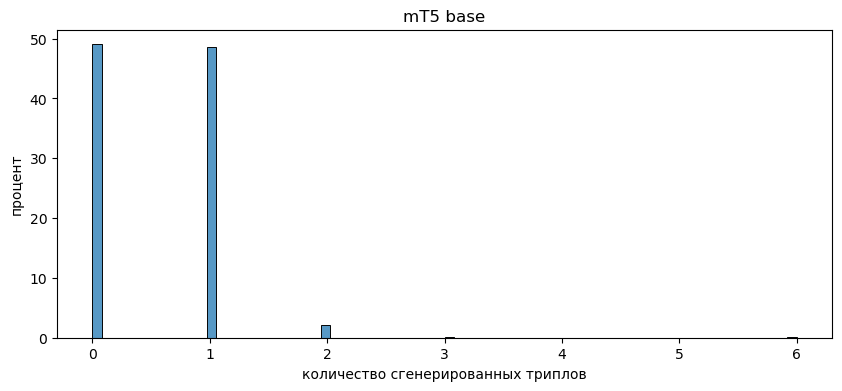
\includegraphics[width=0.9\textwidth]{images/mT5_base_preds_distr.png}
    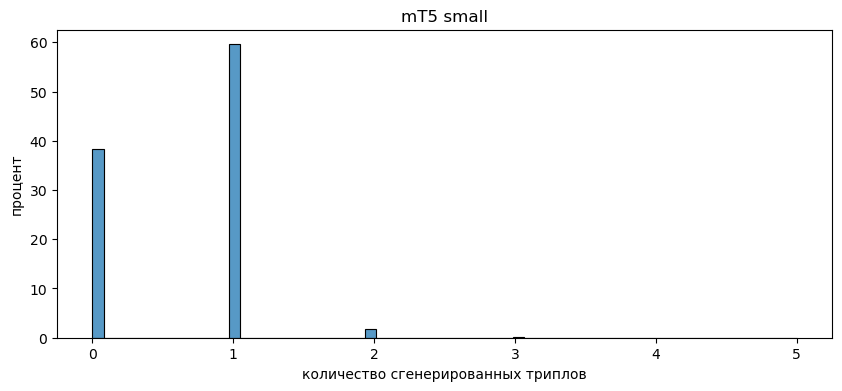
\includegraphics[width=0.9\textwidth]{images/mT5_small_preds_distr.png}
    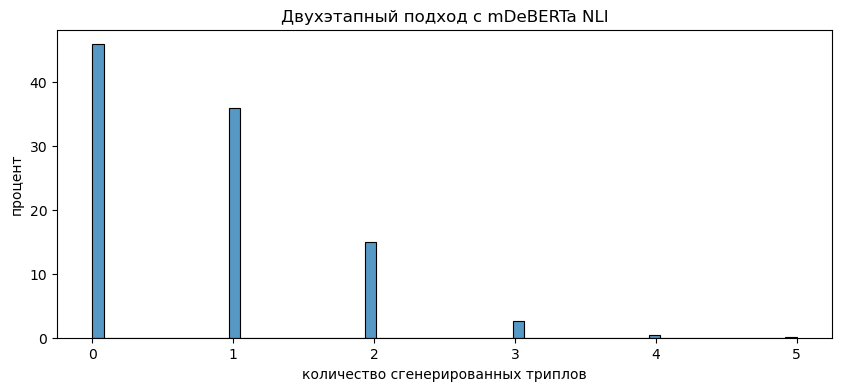
\includegraphics[width=0.9\textwidth]{images/two_stage_preds_distr.png}
    \caption{Распределения количества триплетов в предсказаниях моделей.}
    \label{fig:preds_distr}
\end{figure}

        \newpage
        \section{Применения}

У извлечения пользовательских атрибутов из диалогов в структурированном формате имеется потенциально очень много приложений. Например, можно использовать в поисковиках, в рекомендательных системах друзей, в социальных науках, в персонализованных диалоговых ассистентах и так далее. Причинами проведения данной работы послужили следующие применения: персонализованных диалоговые ассистенты и рекомендательные системы.

\textbf{Персонализованные диалоговые ассистенты}    Огромное внимание уделяется разработке систем, которые могут повысить качество беседы и сделать ее более увлекательной для участников. Есть два направления развития агентов персонализированного диалога: придание агентам индивидуальности как в статье про PersonaChat \cite{personachat}, или адаптация агентов к их конечным пользователям с помощью пользовательских атрибутов. Следовательно, если можно снабдить диалоговую систему модулем извлечения пользовательских атрибутов, это станет шагом в развитии персонализированных диалоговых систем.

Диалоговая система может рассматривать пользовательские атрибуты, извлеченные из истории диалога, как долгосрочную память. Эта информация позволяет избежать системе повторять одни и те же или похожие вопросы. Например, если пользователь упомянул, что он родился в сентябре 2009 года в предыдущем разговоре два дня назад, система персонализированного диалога должна избегать задавать вопросы типа "В каком месяце у вас день рождения?" или "А сколько тебе лет?". Кроме того, такие атрибуты можно использовать для фильтрации ответов системы или для предложения ответов получше. Например, для персонализированной системы было бы неуместно спрашивать "Как у вас дела в универе?", если пользователь родился в 2013м году, в то время как сейчас 2023й год. Лучше будет, если система ответит "Вау! Скоро тебе исполнится 10!" после получения информации о времени рождения пользователя.

\textbf{Персонализованные рекомендательные системы}     Существует три основных типа рекомендательных систем: knowledge-based система содержит атрибуты пользователя и продуктов и дает рекомендации на основе сходства этих атрибутов; content-based система рекомендует товары, похожие тем, которые понравились данному пользователю в прошлом, независимо от предпочтений других пользователей; в то время, как система на основе collaborative-filtering делает рекомендации основываясь на прошлых взаимодействиях всей базы пользователей, например, рассматривая k-ближайших соседей данного пользователя.

Большинство этих рекомендательных систем требуют фактического взаимодействия пользователей с продуктами, такими как щелчок мышью или просмотр. Используя решения из данной работы можно собирать пользовательские атрибуты в неявном режиме, которые затем можно использовать в кластеризации пользователей или для сохранения продуктов упомянутые пользователем в прошлом. Например, если имеются два пользователя и оба из Москвы и любят хоккей, то можно порекомендовать игру ЦСКА одному пользователю, если другой часто упоминает ее.


        \newpage
        \chapter{\centering\normalsize{ЗАКЛЮЧЕНИЕ}}
\addcontentsline{toc}{section}{ЗАКЛЮЧЕНИЕ}

В данной работе было исследовано извлечение атрибутов пользователей из разговорных данных. Из-за отсутствия датасета с качественной разметкой была использована техника distant supervision, которая добавила значительный шум в данные. Тем не менее, почти все методы из этой работы получили результат лучше чем базовая модель, показавшая в использованном датасете самые высокие показатели. Так же были описаны достоинства и недостатки каждого из предложенных подходов, а так же потенциальные применения этих методов. Так же были помечены направления для дальнейшей разработки и исследований.


	\newpage
	\printbibliography

        \newpage
        \appendix
\chapter{\centering\normalsize{ПРИЛОЖЕНИЕ}}
\addcontentsline{toc}{section}{ПРИЛОЖЕНИЕ}
\section{Дополнительные эксперименты на датасете WikiNRE} \label{AppendixA}

Для оценки качества GenAE в случае консистентного порядка триплетов, был рассмотрен датасет WikiNRE собранный на основе данных из Wikipedia и графа знаний Wikidata. В качестве генеративной модели был взят T5 v1.1 small и обучен в течение 4 эпох c AdamW c \texttt{lr=0.00002} и \texttt{weight\_decay=0.01} на 4 картах GeForce GTX 1080 Ti. Размер batch'a на каждое вычислительное устройство равен 16, без learning rate warmup.

Результаты представлены в Tаблице \ref{table:wikinre_results}. Для сравнения брались модели из статьи \cite{genie}, которые являются наиболее популярными в построении графов знаний. Можно увидеть, что с наивным методом обучения GenAE уступает только GenIE с BART-large \cite{bart} и с constrained beam-search \cite{seq2seq}. Тем не менее, GenAE работает лучше всех подходов основанных на нескольких моделях в виде pipeline. Результат GenAE в этом датасете намного выше, так как в нем нет шума и соблюдается порядок триплетов если их несколько во входной реплике. Тем не менее, задача поставленная в датасете схожа с основной задачей данной работы только форматом извлечения информации, а домен полностью отличается: в WikiNRE не разговорный домен и предикаты общие и не относятся к персоне определенного человека.

\begin{table}[!ht]
\centering
\begin{tabular}{c c c c}
    & Precision & Recall & F1 \\
    \hline
    \hline
    NeuralEL + CNN & 36.89 & 35.21 & 36.03 \\
    \hline
    SotA Pipeline & 67.43 & 54.22 & 60.11  \\
    \hline
    GenAE c T5-small & 79.29 & 73.62 & 76.35 \\
    \hline
    GenIE & \textbf{88.18} & \textbf{88.31} & \textbf{88.24}  \\
    \hline
\end{tabular}
\caption{Результаты извлечения триплетов на датасете WikiNRE \cite{trisedya-etal-2019-neural}. Все показатели кроме GenAE взяты из статьи \cite{genie} и \cite{trisedya-etal-2019-neural}.}
\label{table:wikinre_results}
\end{table}

\newpage
\section{Дополнительные эксперименты на датасете DialogueNLI c ChatGPT} \label{AppendixB}

\begin{table}[!ht]
\centering
\begin{tabular}{c c c c c c}
    & Precision & Recall & F1 & Accuracy & BLEU-1 \\
    \hline
    \hline
    ChatGPT & 13.85 & 29.63 & 18.88 & 17.0 & 76.87 \\
    \hline
    GenAE & \textbf{43.14} & 40.74 & 41.9 & \textbf{42.0} & 76.11  \\
    \hline
    PipelineAE & 42.45 & \textbf{54.63} & \textbf{47.77} & 40.0 & \textbf{83.37} \\
    \hline
\end{tabular}
\caption{Результаты извлечения триплетов на датасете DialogueNLI.}
\label{table:chatgpt_results}
\end{table}

\end{document}